% COUNT: 169
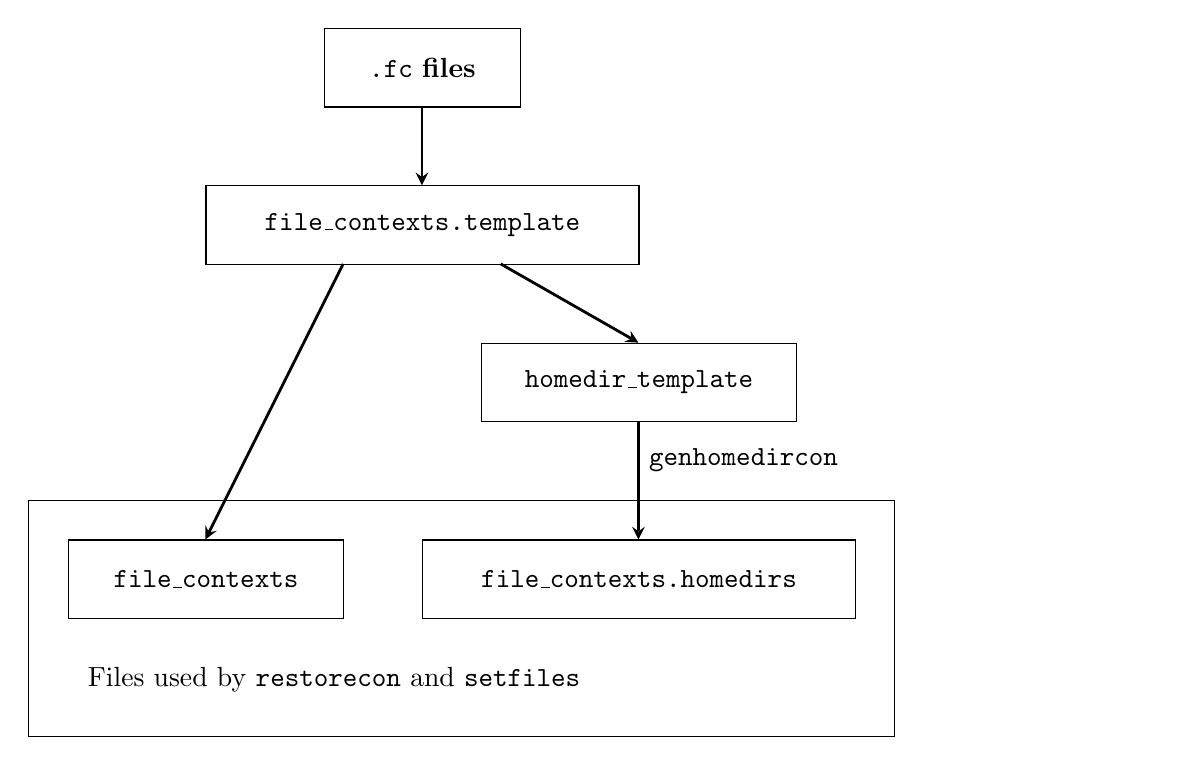
\begin{tikzpicture}
    \usetikzlibrary{calc}
    \tikzstyle{arrow} = [->,>=stealth, line width=1pt]
    \tikzstyle{darrow} = [<->,>=stealth, line width=1pt]
    \tikzstyle{rec} = [rectangle, draw=black, align=center, text width=3.5cm,
        minimum height=1cm, minimum width=4cm, fill=white]

    \draw (0,-6.5) rectangle (11,-9.5);
    %\draw[step=1cm,gray,very thin] (0,0) grid (11,-8);

    \node(fcfiles) [rec, text width=2cm, minimum width=2.5cm]
        at (3.75,-0.5) [anchor=north west]
        {\textbf{\texttt{.fc} files}};

    \node(fctemp) [rec, text width=5cm, minimum width=5.5cm]
        at (2.25,-2.5) [anchor=north west]
        {\textbf{\texttt{file\_contexts.template}}};

    \node(fc) [rec, text width=3cm, minimum width=3.5cm]
        at (0.5,-7) [anchor=north west]
        {\textbf{\texttt{file\_contexts}}};

    \node(hdtemp) [rec, text width=3.5cm, minimum width=4cm]
        at (5.75,-4.5) [anchor=north west]
        {\textbf{\texttt{homedir\_template}}};

    \node(fchd) [rec, text width=5cm, minimum width=5.5cm]
        at (5,-7) [anchor=north west]
        {\textbf{\texttt{file\_contexts.homedirs}}};

    \node(text) [text width=13.5cm, minimum width=14cm]
        at (0.5,-8.5) [anchor=north west]
        {Files used by \texttt{restorecon} and \texttt{setfiles}};

    \draw[arrow] (5,-1.5) -- (5,-2.5);
    \draw[arrow] (4,-3.5) -- (2.25,-7);
    \draw[arrow] (6,-3.5) -- (7.75,-4.5);
    \draw[arrow] (7.75,-5.5) -- node[pos=0.33,right] {\texttt{genhomedircon}}
        (7.75,-7);
\end{tikzpicture}
